\section{Módulo multimedia y aplicación de IA}
\label{sec:multimedia}

Esta sección cubre el enunciado 5.3.1 (representación clásica frente a embeddings
densos), la aplicación vertical de la sección 5.5 (opción A: RAG) y el Experimento 7.
La regla de diseño fue no inventar almacenamiento nuevo: cada representación termina
en una tabla \code{HEAP} con una columna \code{VECTOR(D)} o en el índice invertido de
la sección~\ref{sec:textual}, y cada consulta pasa por el planificador de la
sección~\ref{sec:vectorial} o por los postings en disco, con el \code{DiskCounter}
contando.

\subsection{Dos representaciones de una imagen}

\paragraph{Paradigma clásico: Bag of Visual Words.}
SIFT (OpenCV) produce para cada imagen unos cientos de descriptores locales de 128
dimensiones, invariantes a escala y rotación. Un \emph{codebook} de $K$ palabras
visuales se entrena con K-Means (variante \emph{mini-batch} de scikit-learn) sobre una
muestra estratificada de descriptores de 1\,500 imágenes; después cada descriptor de
cada imagen se cuantiza a su centroide más cercano y la imagen queda representada por
la bolsa \code{["vw0012", "vw0012", "vw0377", \ldots]}. Esa lista entra al mismo SPIMI
que los documentos de texto: \code{build\_index(\ldots, tokenize=identidad)} salta
stopwords y stemming, porque una palabra visual no tiene morfología. La consulta es
TF-IDF logarítmico con similitud de coseno,

\[
  w_{t,d} = (1+\log_{10} tf_{t,d})\cdot\log_{10}\frac{N}{df_t},\qquad
  \mathrm{score}(q,d)=\frac{\sum_{t\in q} w_{t,q}\,w_{t,d}}{\lVert d\rVert_2\,\lVert q\rVert_2},
\]

donde la norma $\lVert d\rVert_2$ se precalcula al construir el índice y se guarda en
disco en \code{<base>.norms.dat}, un archivo paginado de registros
$\langle$page, slot, norma$\rangle$ (16 bytes). Las normas se leen una vez al abrir el
índice y quedan en RAM, con el mismo criterio que los centroides del IVF: son $N$
flotantes y releerlas en cada consulta solo añadiría ruido a la comparación. El
codebook se persiste como la tabla \code{codebook\_bovw(id INT, centro VECTOR(128))},
así que la aplicación lo recupera con un \code{scan} y no hay serializador externo.

\paragraph{Paradigma moderno: embeddings densos.}
ResNet-18 preentrenada en ImageNet, sin la capa de clasificación: el vector de 512
dimensiones del \emph{average pooling}, normalizado a norma 1. Va en la columna
\code{emb VECTOR(512)} de la tabla \code{imagenes(id, categoria CHAR(20), archivo
CHAR(64), emb)} y se indexa con \code{CREATE INDEX idx\_emb ON imagenes (emb) USING IVF
WITH (metric = 'COSINE')}. La consulta es SQL ordinario del módulo vectorial:

\begin{lstlisting}
SELECT id, categoria, archivo, emb <=> '[...]' AS dist
FROM imagenes ORDER BY dist ASC LIMIT 10;      -- IVFScan (o KnnSeqScan con <->)
\end{lstlisting}

\begin{figure}[H]
\centering
\begin{tikzpicture}[
  node distance=3mm and 5mm,
  caja/.style={draw, rounded corners=1pt, align=center, font=\footnotesize, inner sep=3pt, minimum height=7mm},
  flecha/.style={-{Latex[length=1.8mm]}, thick},
]
\node[caja] (img) {imagen};
\node[caja, above right=2mm and 8mm of img, fill=blue!6] (sift) {SIFT\\ $n\times128$};
\node[caja, right=of sift, fill=blue!6] (cb) {codebook\\ K-Means ($K$)\\ tabla \code{codebook\_bovw}};
\node[caja, right=of cb, fill=blue!6] (bag) {bolsa de palabras\\ \code{vw0012 vw0377 \ldots}};
\node[caja, right=of bag, fill=green!6] (inv) {índice invertido\\ vocab B+ + postings\\ + \code{norms.dat}};
\node[caja, below right=2mm and 8mm of img, fill=orange!8] (cnn) {ResNet-18\\ avgpool 512-D};
\node[caja, right=of cnn, fill=orange!8] (tab) {\code{imagenes.emb}\\ \code{VECTOR(512)}};
\node[caja, right=of tab, fill=green!6] (ivf) {IVF COSINE\\ \code{.ivf.dir} + \code{.ivf.lst}};
\node[caja, right=of ivf] (q2) {\code{ORDER BY emb <=> q}\\ \code{LIMIT k}};
\node[caja, right=of inv] (q1) {TF-IDF coseno\\ top-$k$ (heap)};
\draw[flecha] (img) -- (sift); \draw[flecha] (sift) -- (cb); \draw[flecha] (cb) -- (bag); \draw[flecha] (bag) -- (inv); \draw[flecha] (inv) -- (q1);
\draw[flecha] (img) -- (cnn); \draw[flecha] (cnn) -- (tab); \draw[flecha] (tab) -- (ivf); \draw[flecha] (ivf) -- (q2);
\end{tikzpicture}
\caption{Los dos caminos de una imagen. Arriba el clásico (SIFT $\to$ palabras visuales $\to$ índice invertido), abajo el moderno (CNN $\to$ \code{VECTOR} $\to$ IVF). Los dos terminan en archivos paginados del motor.}
\end{figure}

\subsection{Texto: SBERT sobre el mismo motor}

Para el corpus del RAG el embedding es SBERT multilingüe
(\code{paraphrase-multilingual-MiniLM-L12-v2}, 384 dimensiones), calculado sobre
``título. texto'' para que el título pese en la representación. La tabla
\code{documentos(id, lang CHAR(2), titulo CHAR(80), texto CHAR(1000), emb VECTOR(384))}
ocupa un registro por página de 4 KB (2\,622 bytes), lo que hace muy visible la
diferencia entre leer la tabla y leer un índice. Sobre ella conviven el IVF
(\code{idx\_emb}, métrica coseno) y el índice invertido SPIMI construido con el
pipeline léxico del Rol 2, sobre cuyos postings corren tanto BM25 como el TF-IDF
coseno de esta sección. Todos los índices textuales viven en \code{data/text/} porque
el catálogo descubre los índices relacionales por el nombre del archivo y el
vocabulario, que es un B+ de términos, no debe aparecer como un índice de la tabla.

\subsection{Aplicación de IA: RAG sobre Wikipedia}

\paragraph{Corpus.} 15\,000 artículos de Wikipedia (7\,500 en español y 7\,500 en
inglés, dump 20231101 vía la API de filas de Hugging Face), con el inicio de cada
artículo recortado a 1\,000 bytes. El descargador (\code{backend/rag/download.py})
reanuda desde donde quedó el CSV y respeta el límite de tasa del servidor
(HTTP 429) con espera exponencial, porque la API corta alrededor de las 5\,000 filas
seguidas.

\paragraph{Flujo.} Ante una pregunta en lenguaje natural el servicio
(\code{backend/rag/pipeline.py}) ejecuta las dos recuperaciones y las devuelve lado a
lado:

\begin{enumerate}[nosep]
  \item \textbf{léxica}: términos de la consulta $\to$ vocabulario B+ $\to$ solo las
        listas de posteo de esos términos $\to$ TF-IDF coseno (o BM25) $\to$ top-$k$;
  \item \textbf{semántica}: SBERT(pregunta) $\to$ \code{SELECT \ldots ORDER BY emb <=>
        '[\ldots]' LIMIT k} $\to$ el planificador elige \code{IVFScan} (con
        \code{SET ivf.probes}) o \code{KnnSeqScan};
  \item \textbf{prompt}: los $k$ fragmentos numerados (semánticos, léxicos o la fusión
        por rango de ambas listas) más la pregunta, con la instrucción de responder en
        el idioma de la pregunta y citar \code{[n]};
  \item \textbf{generación}: el cliente \code{backend/rag/llm.py} es independiente del
        proveedor (SDK de Anthropic, cualquier API compatible con
        \code{/chat/completions} ---Gemini, Groq, OpenAI, Ollama--- o un modelo local
        con \code{transformers}); sin clave cae a una respuesta \emph{extractiva} que
        mantiene demostrable el resto del pipeline.
\end{enumerate}

El cliente web muestra la respuesta con las citas enlazadas a las fuentes, los
fragmentos de cada ruta con su score y, para cada ruta, la ruta de acceso, la latencia
y los bloques leídos del índice y de la tabla. Es el mismo desglose que exige el
planificador híbrido, aplicado a una aplicación completa.

\paragraph{Interfaz multimedia.} La segunda vista permite subir una foto o elegir una
imagen indexada como consulta y devuelve el top-$k$ de los dos paradigmas con
miniaturas, el tiempo de extracción (SIFT + cuantización frente al paso por la CNN),
la latencia, el I/O y ---cuando la consulta es una imagen del dataset--- la
Precision@$k$ por categoría, marcando en verde los aciertos.

\subsection{Experimento 7: paradigma clásico vs. embeddings densos}

\paragraph{Metodología.} Caltech-101 completo sin la carpeta de fondo (8\,677
imágenes, 101 categorías). Consultas: 5 imágenes al azar de cada una de las 30
categorías más pobladas (150 consultas); una imagen recuperada es relevante si tiene la
categoría de la consulta y la propia consulta se excluye del ranking. Métodos: BoVW con
$K\in\{128,256,512\}$ sobre el índice invertido con TF-IDF coseno; ResNet-18 con k-NN
exacto (\code{KnnSeqScan}, verdad de campo del IVF) y con IVF y
\code{probes}$\in\{1,5,20\}$. Se mide Precision@5, Precision@10, el tiempo de
extracción por imagen (SIFT + cuantización frente al \emph{forward} por lotes de la
CNN), la latencia de consulta y los bloques leídos del índice y de la tabla. El bloque
7b repite la comparación en texto con una búsqueda de ítem conocido sobre Wikipedia
(consulta = título del artículo): TF-IDF coseno y BM25 frente a SBERT exacto e IVF.

\begin{table}[H]
\centering\footnotesize\setlength{\tabcolsep}{4pt}
\begin{tabular}{lrrrrrrr}
\toprule
Método & P@5 (\%) & P@10 (\%) & extracción (ms/img) & consulta (ms) & bloques & índice / tabla & índice (KB) \\
\midrule
BoVW, $K=128$ & 10,8 & 8,8 & 11,9 & 971,1 & 2\,703 & 2\,692 / 11 & 13\,132 \\
BoVW, $K=256$ & 14,4 & 12,5 & 11,9 & 1\,057,5 & 3\,085 & 3\,074 / 11 & 19\,292 \\
BoVW, $K=512$ & 19,3 & 16,5 & 11,6 & 964,8 & 2\,928 & 2\,917 / 11 & 25\,240 \\
ResNet-18, k-NN exacto & 87,1 & 85,9 & 17,2 & 358,6 & 8\,677 & 0 / 8\,677 & 0 \\
ResNet-18, IVF probes=1 & 86,3 & 85,7 & 17,2 & 6,0 & 117 & 106 / 11 & 35\,088 \\
ResNet-18, IVF probes=5 & 87,3 & 86,5 & 17,2 & 13,4 & 509 & 498 / 11 & 35\,088 \\
ResNet-18, IVF probes=20 & 87,2 & 86,0 & 17,2 & 39,2 & 1\,880 & 1\,869 / 11 & 35\,088 \\
\bottomrule
\end{tabular}
\caption{Experimento 7a (\code{exp7\_imagenes.csv}): Caltech-101, 8677 imágenes de 101 categorías, 150 consultas. Precisión = fracción del top-$k$ con la misma categoría que la consulta (sin contar la propia imagen).}
\label{tab:exp7a}
\end{table}

\begin{table}[H]
\centering\footnotesize\setlength{\tabcolsep}{4pt}
\begin{tabular}{lrrrrrrr}
\toprule
Método & hit@1 (\%) & hit@10 (\%) & MRR@10 & consulta$\to$vector (ms) & búsqueda (ms) & bloques & índice / tabla \\
\midrule
TF-IDF + coseno & 77,3 & 96,3 & 0,844 & 0,1 & 1,6 & 16 & 9 / 7 \\
BM25 & 84,7 & 96,7 & 0,892 & 0,1 & 1,5 & 16 & 9 / 7 \\
SBERT, k-NN exacto & 77,3 & 89,3 & 0,820 & 11,4 & 158,5 & 4\,000 & 0 / 4\,000 \\
SBERT, IVF probes=1 & 48,3 & 54,3 & 0,507 & 10,3 & 5,8 & 48 & 38 / 10 \\
SBERT, IVF probes=5 & 68,3 & 77,0 & 0,720 & 10,2 & 9,0 & 191 & 181 / 10 \\
SBERT, IVF probes=20 & 75,0 & 86,7 & 0,795 & 10,7 & 20,8 & 674 & 664 / 10 \\
\bottomrule
\end{tabular}
\caption{Experimento 7b (\code{exp7\_texto.csv}): Wikipedia es/en, 4000 artículos, 300 consultas de ítem conocido (la consulta es el título; acierto = recuperar ese artículo).}
\label{tab:exp7b}
\end{table}


\begin{figure}[H]
\centering
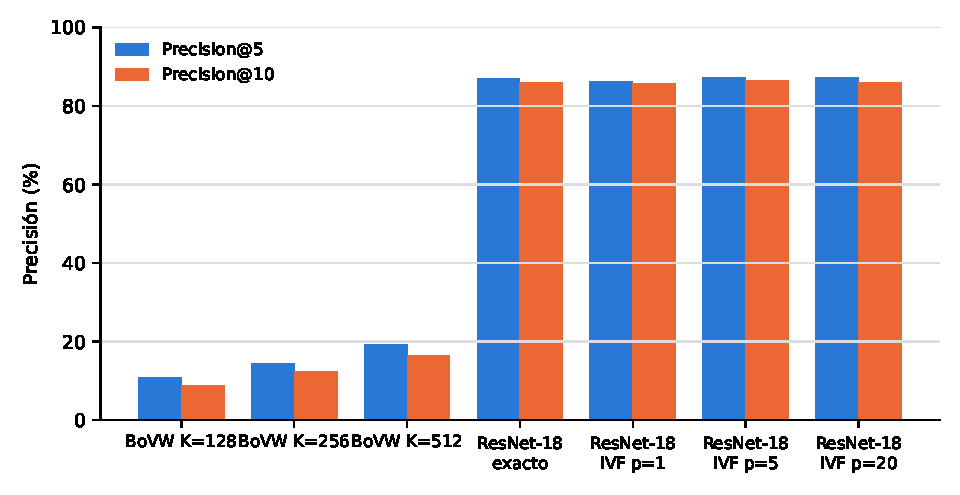
\includegraphics[width=0.85\textwidth]{exp7_precision}
\caption{Precision@5 y @10 por método en Caltech-101.}
\end{figure}

\begin{figure}[H]
\centering
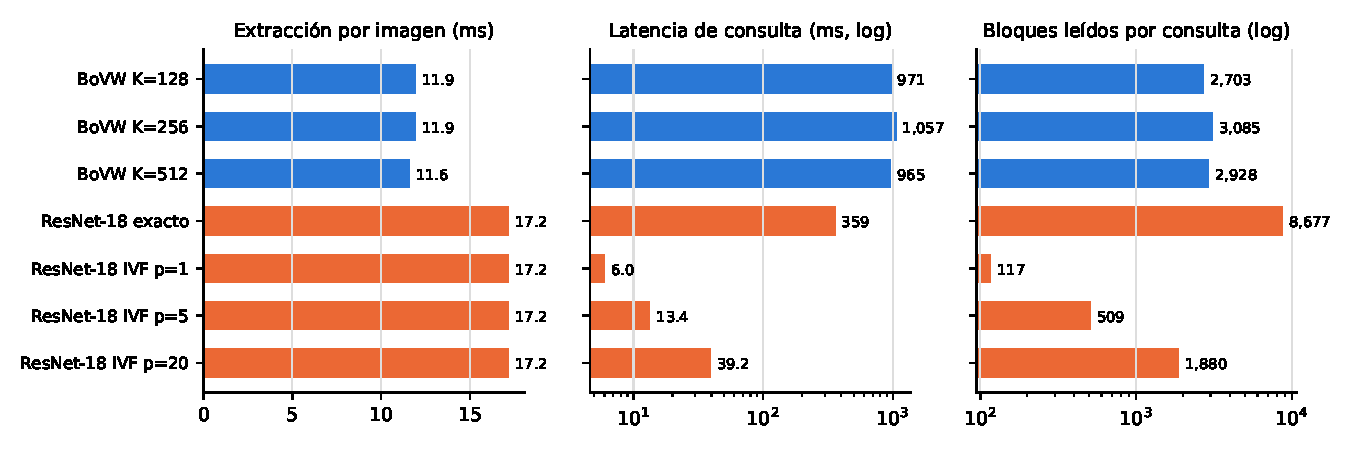
\includegraphics[width=\textwidth]{exp7_costos}
\caption{Costo de cada método: extracción por imagen, latencia de consulta y bloques leídos (escala logarítmica donde la diferencia lo exige).}
\end{figure}

%%ANALISIS7A%%

\begin{figure}[H]
\centering
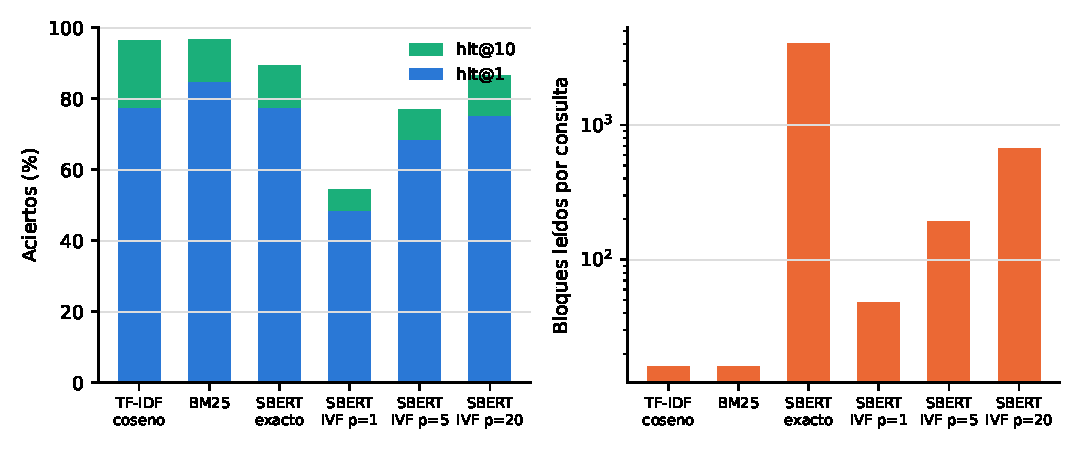
\includegraphics[width=0.9\textwidth]{exp7_texto}
\caption{Experimento 7b: aciertos de ítem conocido y bloques leídos por consulta, léxico frente a SBERT.}
\end{figure}

%%ANALISIS7B%%
